\documentclass{article}%
\usepackage[T1]{fontenc}%
\usepackage[utf8]{inputenc}%
\usepackage{lmodern}%
\usepackage{textcomp}%
\usepackage{lastpage}%
\usepackage[tmargin=1cm,lmargin=10cm]{geometry}%
\usepackage{amsmath}%
\usepackage{tikz}%
\usepackage{pgfplots}%
\pgfplotsset{compat=newest}%
\usepackage{graphicx}%
%
%
%
\begin{document}%
\normalsize%
\section{The simple stuff}%
Some regular text and some%
\textit{italic text. }%
\newline%
Also some crazy characters: \$\&\#\{\}%
\subsection{Math that is incorrect}%
\[%
2*3 = 9%
\]

%
\subsection{Table of something}%
\begin{tabular}{rc|cl}%
\hline%
1&2&3&4\\%
\cline{1%
-%
2}%
&&&\\%
4&5&6&7\\%
\end{tabular}

%
\section{The fancy stuff}%
\subsection{Correct matrix equations}%
\[%
\begin{pmatrix}%
2&3&4\\%
0&0&1\\%
0&0&2%
\end{pmatrix} \begin{pmatrix}%
100\\%
10\\%
20%
\end{pmatrix} = \begin{pmatrix}%
310\\%
20\\%
40%
\end{pmatrix}%
\]

%
\subsection{Alignat math environment}%
\begin{alignat*}{2}%
\frac{a}{b} &= 0 \\%
\begin{pmatrix}%
2&3&4\\%
0&0&1\\%
0&0&2%
\end{pmatrix}%
\begin{pmatrix}%
100\\%
10\\%
20%
\end{pmatrix}%
&=%
\begin{pmatrix}%
310\\%
20\\%
40%
\end{pmatrix}%
\end{alignat*}

%
\subsection{Beautiful graphs}%
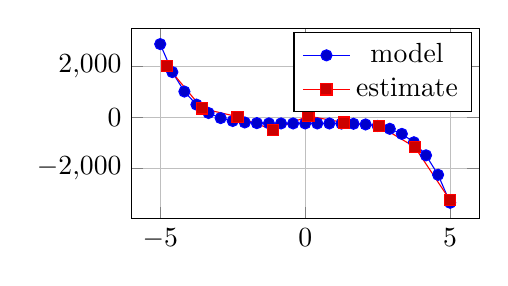
\begin{tikzpicture}%
\begin{axis}[height=4cm, width=6cm, grid=major]%
\addplot{-x^5 - 242};%
%
\addlegendentry{model}%
\addplot coordinates {%
(-4.77778,2027.60977)%
(-3.55556,347.84069)%
(-2.33333,22.58953)%
(-1.11111,-493.50066)%
(0.11111,46.66082)%
(1.33333,-205.56286)%
(2.55556,-341.40638)%
(3.77778,-1169.2478)%
(5.0,-3269.56775)%
};%
%
\addlegendentry{estimate}%
\end{axis}%
\end{tikzpicture}

%
\subsection{Cute kitten pictures}%


\begin{figure}[h!]%
\centering%

\includegraphics[width=120px]{/Users/rparayno/Projects/dlsuresumegenerator/latexgenerate/icon.png}%
\caption{Look it's on its back}%
\end{figure}

%
\end{document}